\chapter{Implementasi dan Pengujian}
\label{chap:implementasidanpengujian}
Bab ini akan membahas hasil implementasi dalam pengembangan perangkat lunak KIRI berdasarkan rancangan yang telah dibuat pada Bab \ref{chap:perancangan}. Selain itu, akan dibahasa juga mengenai pengujian dari perangkat lunak KIRI yang sudah dikembangkan.
\section{Implementasi}
\label{sec:implementasi}
Pada bagian ini akan dijelaskan mengenai lingkungan implementasi perangkat lunak yang telah dikembangkan beserta hasilnya. Bagian ini terbagi menjadi empat subbagian, yaitu lingkungan perangkat keras, lingkungan perangkat keras, hasil implementasi antarmuka, dan hasil implementasi antarmuka. Implementasi perangkat lunak ini didasarkan pada perancangan yang telah dijelaskan pada Bab \ref{chap:perancangan}.

\subsection{Lingkungan Perangkat Keras}
\label{subsec:lingkunganperangkatkeras}
Perangkat keras yang digunakan dalam mengimplementasi rancangan perangkat lunak memiliki spesifikasi sebagai berikut:
\begin{enumerate}
    \item Laptop: ASUS TUF Gaming F15
    \item \textit{Processor}: Intel(R) Core(TM) i7-12700H (20 CPUs), 2.3GHz
    \item \textit{Random Access Memory} (RAM): 16GB
    \item \textit{Solid State Drive} (SSD): 512GB
\end{enumerate}

\subsection{Lingkungan Perangkat Lunak}
\label{subsec:lingkunganperangkatlunak}
Perangkat lunak yang digunakan dalam mengimplementasi rancangan perangkat lunak memiliki spesifikasi sebagai berikut:
\begin{enumerate}
    \item \textit{Operating System}: Windows 11 Home Single Language
    \item Bahasa Pemrograman:
    \begin{itemize}
        \item PHP
        \item Java
        \item Javascript
    \end{itemize}
    \item Framework: CodeIgniter 3.1.13
    \item Code Editor: Visual Studio Code 1.99.3
    \item Perangkat Lunak Pendukung:
    \begin{itemize}
        \item XAMPP version 3.3.0
        \item phpMyAdmin 5.2.1
        \item Apache Ant 1.10.15
        \item PHP 8.2.12
        \item Java 19.0.2
    \end{itemize}
\end{enumerate}

\newpage
\subsection{Penjelasan Kode Program}
\label{subsec:penjelasankode}
Pada bagian ini akan dijelaskan kode-kode program atau kelas-kelas yang telah diimplementasikan untuk mendungkung pengembangan perangkat lunak KIRI. Kode-kode program tersebut mencakup kode program yang baru saja ditambahkan serta kode program yang sudah ada sejak awal dan dilakukan modifikasi. Berikut merupakan penjelasannya.

\subsubsection{Dijkstra.java}
Kelas ini berfungsi untuk mengimplementasikan algoritma Dijkstra yang digunakan untuk mencari jalur terpendek dari satu titik ke titik lainnya dalam graf berbobot. Secara keseluruhan kelas Dijkstra masih sama seperti yang dijelaskan di \ref{subss:dijkstra}.
\\
Pada kelas Dijkstra ini, hanya dilakukan sedikit perubahan dari implementasi aslinya (lihat Kode \ref{code:dijkstra}). Perubahan yang dilakukan hanya menambahkan pewarisan (extends ShortestPathStrategy) agar kelas Dijkstra dapat menjadi turunan dari kelas abstrak ShortestPathStrategy, yang berfungsi sebagai kerangka umum untuk berbagai algoritma pencarian jalur. 

\begin{lstlisting}[language=Java, caption=Dijkstra.java, basicstyle=\small\ttfamily]
    public class Dijkstra extends ShorestPathStrategy
\end{lstlisting}
\noindent
Selain itu, beberapa \textit{method} di dalam kelas ini diberi anotasi \texttt{@Override} untuk menandakan bahwa metode tersebut mengimplementasikan metode dari kelas induknya.
\begin{lstlisting}[language=Java, caption=Dijkstra.java, basicstyle=\small\ttfamily]
    @Override
    public double runAlgorithm

    @Override
    public int getParent

    @Override
    public double getDistance
\end{lstlisting}

\noindent
Perubahan lainnya, yaitu memindahkan atribut-atribut utama seperti \texttt{graph}, \texttt{startNode}, \texttt{finishNode}, \texttt{multiplierWalking}, dan \texttt{penaltyTransfer} ke kelas induknya sehingga pemanggilan atribut menggunakan \texttt{super}.

\begin{lstlisting}[language=Java, caption=Dijkstra.java, basicstyle=\small\ttfamily]
 super(graph, startNode, finishNode, multiplierWalking, penaltyTransfer);
\end{lstlisting}

\subsubsection{AStar.java}
Kelas ini adalah implementasi dari algoritma A-Star, yang digunakan untuk mencari jarak terpendek antara dua titik dalam sebuah graf dengan mempertimbangkan heuristic (estimasi jarak ke tujuan). Algoritma ini bekerja dengan mencari rute optimal berdasarkan kombinasi antara jarak yang telah ditempuh (g) dan estimasi jarak yang tersisa (f = g + h). Kode program dari AStar.java bisa dilihat pada lampiran \ref{code:astar} dan berikut merupakan penjelasan dari kode tersebut.
\newpage
\begin{itemize}
    \item \textbf{Atribut}
    \begin{itemize}
        \item \texttt{graph}
        \\ Daftar node dalam graf yang merepresentasikan jaringan jalur. Atribut ini merupakan turunan dari kelas induk / \textit{superclass}
        \item \texttt{startNode} dan \texttt{finishNode}
        \\ Indeks node awal dan akhir dari pencarian. Atribut ini merupakan turunan dari kelas induk / \textit{superclass}
        \item \texttt{nodeInfoLinks}
        \\ Array \texttt{NodeInfo} yang menyimpan informasi seperti jarak yang telah ditempuh (g), estimasi total biaya (f), dan node asal (parent) untuk setiap node.
        \item \texttt{openSet}
        \\ \textit{Priority queue} yang berisi \texttt{NodeInfo} dan mengurutkan node berdasarkan nilai estimasi total biaya (f).
        \item \texttt{multiplierWalking} dan \texttt{penaltyTransfer}
        \\ Faktor pengali dan penalti yang digunakan untuk menghitung bobot tambahan pada node yang terkait dengan jalur pejalan kaki atau perpindahan angkot. Atribut ini merupakan turunan dari kelas induk / \textit{superclass}
    \end{itemize}

    \item \textbf{Method}
    \begin{itemize}
        \item \texttt{runAlgorithm(Set<String> trackTypeIdBlacklist)}
        \\ Method utama untuk menjalankan algoritma. Langkah pertama adalah mengatur jarak dari node awal (g) menjadi 0 dan menghitung estimasi awal (f) menggunakan fungsi heuristic. Node awal kemudian dimasukkan ke dalam openSet. Selama openSet tidak kosong, node dengan nilai f terendah diambil sebagai current. Jika node ini adalah finishNode, maka jarak terpendek (g) dikembalikan. Untuk setiap tetangga dari current, dihitung biaya baru menuju node tersebut menggunakan calculateWeight. Jika biaya baru lebih kecil daripada nilai g yang telah tersimpan, nilai-nilai dalam NodeInfo diperbarui dan node dimasukkan ke openSet. Jika tidak ditemukan jalur ke finishNode, nilai Double.POSITIVE\_INFINITY dikembalikan. Method ini diberi anotasi \texttt{@Override} karena method ini mengimplementasikan method dari kelas induk / \textit{superclass}.

        \item \texttt{getParent(int node)}
        \\ Mengembalikan parent (node asal) dari node yang dimaksud dalam rute terpendek. Method ini diberi anotasi \texttt{@Override} karena method ini mengimplementasikan method dari kelas induk / \textit{superclass}.

        \item \texttt{getDistance(int node)}
        \\ Mengembalikan jarak dari node awal ke node yang diminta (nilai g dari node tersebut). Method ini diberi anotasi \texttt{@Override} karena method ini mengimplementasikan method dari kelas induk / \textit{superclass}.

        \item \texttt{heuristic(int node)}
        \\ Fungsi \textit{heuristic} yang mengembalikan estimasi jarak antara node saat ini dan node tujuan menggunakan metode \texttt{distanceTo} antar koordinat \texttt{LatLon}.

        \item \texttt{calculateWeight(NodeInfo currentNode, GraphEdge edge)}
        \\ Method ini menghitung bobot perjalanan dari \texttt{currentNode} ke node tujuan melalui sebuah edge. Jika salah satu track merupakan jalur pejalan kaki, maka bobot dihitung berdasarkan \texttt{multiplierWalking}. Jika perpindahan kendaraan terjadi, maka bobot ditambah \texttt{penaltyTransfer}. Jika tetap berada dalam kendaraan yang sama, bobot dikalikan dengan penalti jalur tersebut. Method ini mengembalikan nilai \texttt{double} sebagai bobot perjalanan.
    \end{itemize}
\end{itemize}
\newpage
\subsubsection{AStar.NodeInfo}
Merupakan \textit{static nested clas}s yang menyimpan informasi-informasi berikut ini:
\begin{itemize}
    \item \texttt{index}
    \\ Indeks node
    \item \texttt{g}
    \\ Jarak dari node awal ke node ini.
    \item \texttt{f}
    \\ Estimasi total jarak (g + heuristic).
    \item \texttt{parent}
    \\ Node asal yang menuju ke node ini.
\end{itemize}
\noindent
Kelas ini juga mengimplementasikan \texttt{Comparable<NodeInfo>} agar dapat digunakan dalam mengurutkan PriorityQueue berdasarkan nilai f.

\subsubsection{FloydWarshall.java}
Kelas ini merupakan implementasi dari algoritma Floyd-Warshall, yaitu algoritma pemrograman dinamis yang digunakan untuk mencari jarak terpendek antar semua pasangan node dalam graf. Algoritma ini sangat efisien untuk graf yang padat dan tidak bergantung pada struktur heap atau antrian prioritas, melainkan menggunakan matriks jarak. Kode program dari FloydWarshall.java bisa dilihat pada lampiran \ref{code:floydwarshall} dan berikut merupakan penjelasan dari kode tersebut.

\begin{itemize}
    \item \textbf{Atribut}
    \begin{itemize}
        \item \texttt{graph}
        \\ Daftar node dalam graf yang merepresentasikan jaringan jalur. Atribut ini merupakan turunan dari kelas induk / \textit{superclass}.
        \item \texttt{startNode} dan \texttt{finishNode}
        \\ Menyimpan indeks node awal dan akhir untuk pencarian rute spesifik. Atribut ini merupakan turunan dari kelas induk / \textit{superclass}
        \item \texttt{numOfNodes}
        \\ Menyimpan jumlah total node dalam graf.
        \item \texttt{dist}
        \\ Matriks dua dimensi double[][] yang menyimpan jarak terpendek antar setiap pasangan node.
        \item \texttt{parent}
        \\ Matriks dua dimensi int[][] yang menyimpan node asal dari jalur terpendek antara setiap pasangan node.
        \item \texttt{multiplierWalking} dan \texttt{penaltyTransfer}
        \\ Digunakan untuk menghitung bobot perjalanan tambahan yang melibatkan jalan kaki atau perpindahan antar angkot.  Atribut ini merupakan turunan dari kelas induk / \textit{superclass}
    \end{itemize}

    \item \textbf{Method}
    \begin{itemize}
        \item \texttt{runAlgorithm(Set<String> trackTypeIdBlacklist)}
        \\ Method utama untuk menjalankan algoritma. Pertama-tama, semua nilai dalam matriks \texttt{dist} diinisialisasi dengan jarak langsung antar node berdasarkan edge yang tersedia, dan mempertimbangkan blacklist dari \texttt{trackTypeIdBlacklist}. Nilai \texttt{parent[i][j]} diatur sesuai asal hubungan. Kemudian, algoritma berjalan dalam tiga \textit{looping} (\texttt{k}, \texttt{i}, \texttt{j}) untuk mengevaluasi apakah melalui node \texttt{k} bisa memberikan jalur lebih pendek antara \texttt{i} dan \texttt{j}. Jika ya, nilai \texttt{dist[i][j]} dan \texttt{parent[i][j]} diperbarui. Method ini jarak terpendek dari \texttt{startNode} ke \texttt{finishNode}. Method ini diberi anotasi \texttt{@Override} karena method ini mengimplementasikan method dari kelas induk / \textit{superclass}.
\newpage
        \item \texttt{calculateWeight(int fromIndex, GraphEdge edge)}
        \\ Menghitung bobot perjalanan antara dua node berdasarkan jenis track. Jika salah satu track adalah pejalan kaki, bobot dikalikan dengan \texttt{multiplierWalking}. Jika terdapat perpindahan antar kendaraan (track berbeda), penalti \texttt{penaltyTransfer} ditambahkan ke bobot. Jika berada dalam kendaraan yang sama, bobot dikalikan penalti jalur.

        \item \texttt{getParent(int node)}
        \\ Mengembalikan parent (node asal) dari node yang dimaksud dalam rute terpendek dari \texttt{startNode}. Method ini diberi anotasi \texttt{@Override} karena method ini mengimplementasikan method dari kelas induk / \textit{superclass}.

        \item \texttt{getDistance(int node)}
        \\ Mengembalikan jarak terpendek dari \texttt{startNode} ke node yang diminta berdasarkan matriks \texttt{dist}. Method ini diberi anotasi \texttt{@Override} karena method ini mengimplementasikan method dari kelas induk / \textit{superclass}.
    \end{itemize}
\end{itemize}

\subsubsection{ShortestPathStrategy.java}
Kelas ini adalah kelas abstrak yang digunakan sebagai kelas induk untuk berbagai implementasi algoritma \textit{shortest path}, yaitu Dijkstra, A-Star, dan Floyd-Warshall. Kelas ini mengimplementasikan pola desain Strategy Pattern, di mana berbagai algoritma dapat diimplementasikan sebagai subclass dari kelas ini. Tujuannya adalah agar algoritma dapat digunakan secara fleksibel. Kelas ini juga memiliki atribut-atribut yang diturunkan ke subclassnya dan juga method-method yang diimplementasikan pada subclassnya. Kode program kelas ini bisa dilihat pada lampiran \ref{code:sps}.

\subsubsection{Worker.java}
Kelas ini bertanggung jawab untuk menangani permintaan routing (pencarian rute) menggunakan algoritma pencarian jalur terpendek. Secara keseluruhan kelas Worker masih sama seperti yang dijelaskan di \ref{subss:worker}.
\\
Perubahan yang dilakukan pada Worker hanya sedikit dari implementasi aslinya (lihat Kode \ref{code:worker}). Salah satu perubahan yang dilakukan adalah pada method \texttt{findRoute} ketika melakukan pemanggilan method pada kelas algoritma \textit{shortest path}.
\begin{lstlisting}[language=Java, caption=Worker.java, basicstyle=\small\ttfamily]
    ShorestPathStrategy strategy;

    if ("floydwarshall".equals(algorithm)) {
        strategy = new FloydWarshall(vNodes, startNode, endNode, customMultiplierWalking, customPenaltyTransfer);
	} else if ("astar".equals(algorithm)) {
	   strategy = new AStar(vNodes, startNode, endNode, customMultiplierWalking, customPenaltyTransfer);
	} else {
		strategy = new Dijkstra(vNodes, startNode, endNode, customMultiplierWalking, customPenaltyTransfer);
	}

    strategy.runAlgorithm(trackTypeIdBlacklist);
\end{lstlisting}
\noindent
Pada saat ini kelas yang dipanggil merupakan kelas induk, yaitu kelas \texttt{ShortestPathStrategy} yang pada sebelumnya langsung memanggil kelas Dijkstra. Selain itu ada kondisi untuk mendukung pemilihan algoritma yang akan digunakan dalam perhitungan. Selain itu ditambahkan juga baris kode untuk mencatat waktu proses dari perhitungan.

\subsubsection{ServiceListener.java}
Kelas ini bertanggung jawab untuk menangani permintaan layanan pada server KIRI. Kelas ini menerima permintaan HTTP untuk mencari rute dan transportasi terdekat berdasarkan parameter yang diberikan seperti yang sudah dijelaskan di \ref{subss:servicelistener}. Pada kelas ini perubahan yang dilakukan hanya menambah satu parameter saja, yaitu parameter \texttt{PARAMETER\_ALGO} yang diperlukan untuk pemilihan algoritma yang akan digunakan dalam perhitungan. Kode program kelas ini bisa dilihat pada lampiran \ref{code:sl}.


\subsubsection{main.php}
Kelas ini bertanggung jawab sebagai antarmuka dari perangkat lunak KIRI. Perubahan yang dilakukan pada kelas ini yaitu dengan menambahkan baris kode untuk sebuah \textit{dropdown} baru untuk memilih algoritma. Berikut merupakan baris kode yang ditambahkan.

\begin{lstlisting}[language=Java, caption=main.php, basicstyle=\small\ttfamily]
<div class="row p-0">
	<div class="col-lg-12">
		<select id="selectAlgo" class="form-control hidden"></select>
	</div>
</div>
<div class="row p-1">
	<div class="col-3">
		<span for="algoselect" class="align-middle">Algorithm:</span>
	</div>
	<div class="col-9">
		<select id="algoselect" class="form-control">
			<option value="dijkstra">Dijkstra</option>
			<option value="floydwarshall">Floyd-Warshall</option>
			<option value="astar">A*</option>
		</select>
	</div>
</div>
\end{lstlisting}
\noindent
Untuk keseluruhan kode program dari kelas main.php bisa dilihat pada lampiran \ref{code:mainphp}.
\subsubsection{main.js}
main.js merupakan sebuah file skrip JavaScript yang menangani berbagai interaksi antara pengguna dan aplikasi di sisi frontend, seperti mengambil input dari pengguna, menanggapi klik tombol, serta menampilkan hasil pencarian atau rute yang diterima dari server. Perubahan yang dilakukan pada skrip ini terdapat pada \textit{function} \texttt{checkCoordinatesThenRoute} yang dimana ditambahkan satu parameter baru yaitu parameter untuk memilih algoritma yang diambil dari antarmuka. Kode program dari skrip main.js dapat dilihat pada lampiran \ref{code:mainjs}

\subsubsection{protocol.js}
Kelas ini merupakan sebuah kelas JavaScript yang bertugas untuk mengirimkan permintaan data dari sisi pengguna (\textit{frontend}) ke server (\textit{backend}) melalui metode AJAX. Kelas ini memfasilitasi komunikasi antara antarmuka pengguna dengan API. Perubahan dilakukan pada saat mendefinisikan fungsi bernama \texttt{findroute} yaitu menambahkan sebuah parameter baru yaitu parameter \texttt{algo}. Kode program dari kelas ini dapat dilihat pada lampiran \ref{code:protocol}

\subsubsection{Api.php}
Kelas ini adalah sebuah kelas di sisi server (\textit{backend}), yang berperan penting dalam memproses dan menangani setiap permintaan yang dikirimkan oleh pengguna melalui antarmuka aplikasi. Kelas ini akan menerima parameter permintaan, mengeksekusi logika tertentu berdasarkan jenis permintaan tersebut, dan mengembalikan hasil dalam bentuk data JSON. Perubahan yang dilakukan yaitu penambahan parameter baru pada \textit{function} \texttt{\_findroute} dengan menambahkan parameter \texttt{algo}. Kode program dari kelas ini dapat dilihat pada lampiran \ref{code:api}

\subsection{Implementasi Antarmuka}
\label{subsec:penjelasankode}
\begin{figure}[H]
    \centering
    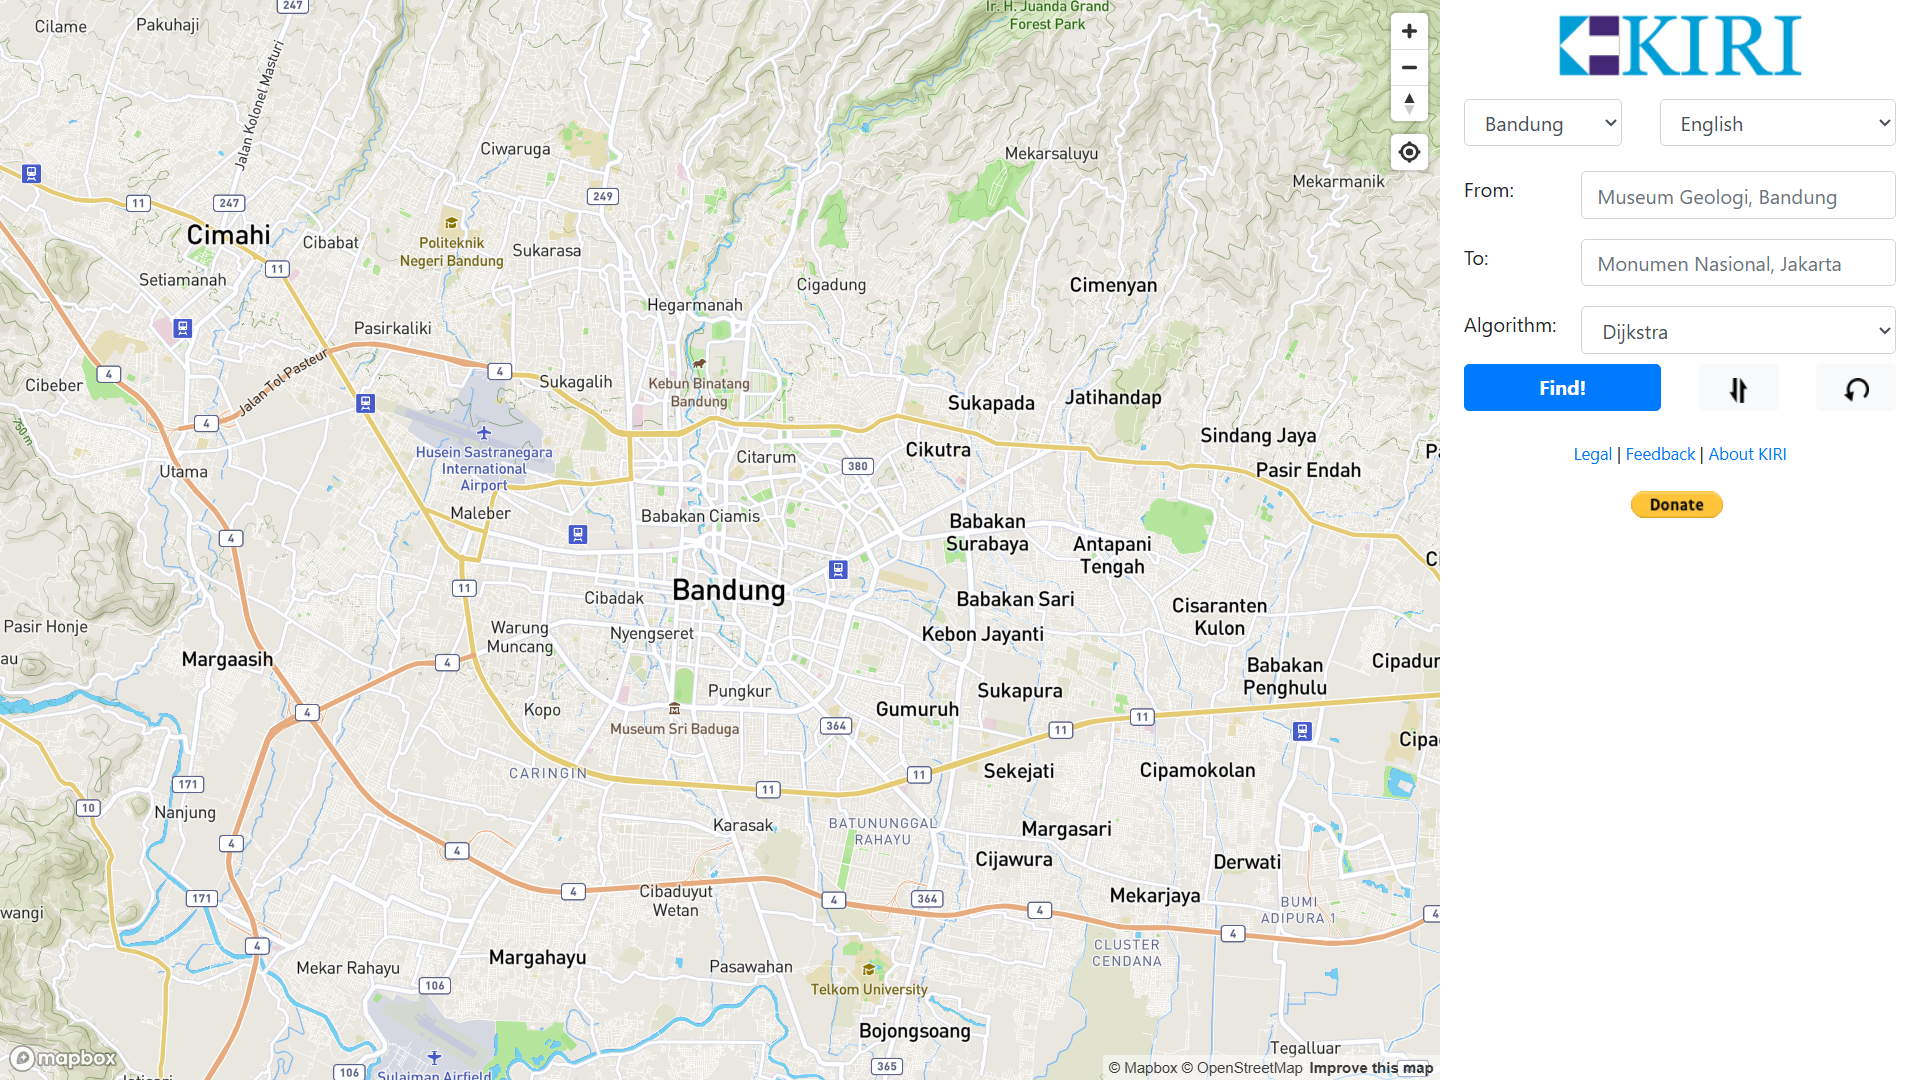
\includegraphics[width=1\textwidth]{antarmuka}
    \caption{Hasil Implementasi Antarmuka}
    \label{fig:antarmuka}
\end{figure}

\noindent
Hasil implementasi perubahan antarmuka dari perangkat lunak KIRI dapat dilihat pada Gambar \ref{fig:antarmuka}. Pengguna dapat memilih salah satu dari tiga algoritma \textit{shortest path} yang ada, yaitu Dijkstra, A-Star, dan Floyd-Warshall pada \textit{dropdown} "\textit{Algorithm}". Sistem akan melakukan pencarian jalur terpendek menggunakan algoritma yang dipilih pengguna.

\section{Pengujian Fungsional dan Eksperimental}
\label{sec:pengujian}
Pada bagian ini akan dijelaskan mengenai hasil pengujian dari perangkat lunak KIRI. Pengujian akan dibagi menjadi dua, yaitu pengujian fungsional dan pengujian eksperimental.

\subsection{Pengujian Fungsional}
\label{subsec:pengujianfungsional}
Pengujian dilakukan dengan tujuan untuk memastikan setiap fungsi pada perangkat lunak KIRI dapat bekerja dengan baik. Pengujian ini dilakukan pada fitur dari perangkat lunak KIRI, dimulai dari, memasukan titik awal dan titik tujuan, dan memilih algoritma yang akan digunakan untuk melakukan pencarian yang merupakan sebuah fitur yang baru diimplementasikan.
\\
Sebelum dilakukan pengujian tersebut, akan dilakukan terlebih dahulu pengujian untuk algoritma FloydWarshall saja. Pengujian dilakukan bertujuan untuk mencari jumlah maksimal dari data "tracks" yang dapat digunakan karena pada saat ini apabila seluruh data "tracks" digunakan maka akan terjadi "java.lang.OutOfMemoryError" yang disebabkan jumlah data "tracks" yang berisikan jalur-jalur transportasi umum dalam bentuk graf terlalu banyak. Jumlah record yang terdapat pada data "tracks" adalah 140 dan pada saat pengujian akan dikurangi 10 record setiap kali pengujiannya hingga algortma Floyd-Warshall dapat berjalan dengan baik. Pengujian ini dilakukan dengan menggunakan Paskal 23 sebagai titik awal dan UNPAR sebagai titik tujuan.

\begin{figure}[H]
    \centering
    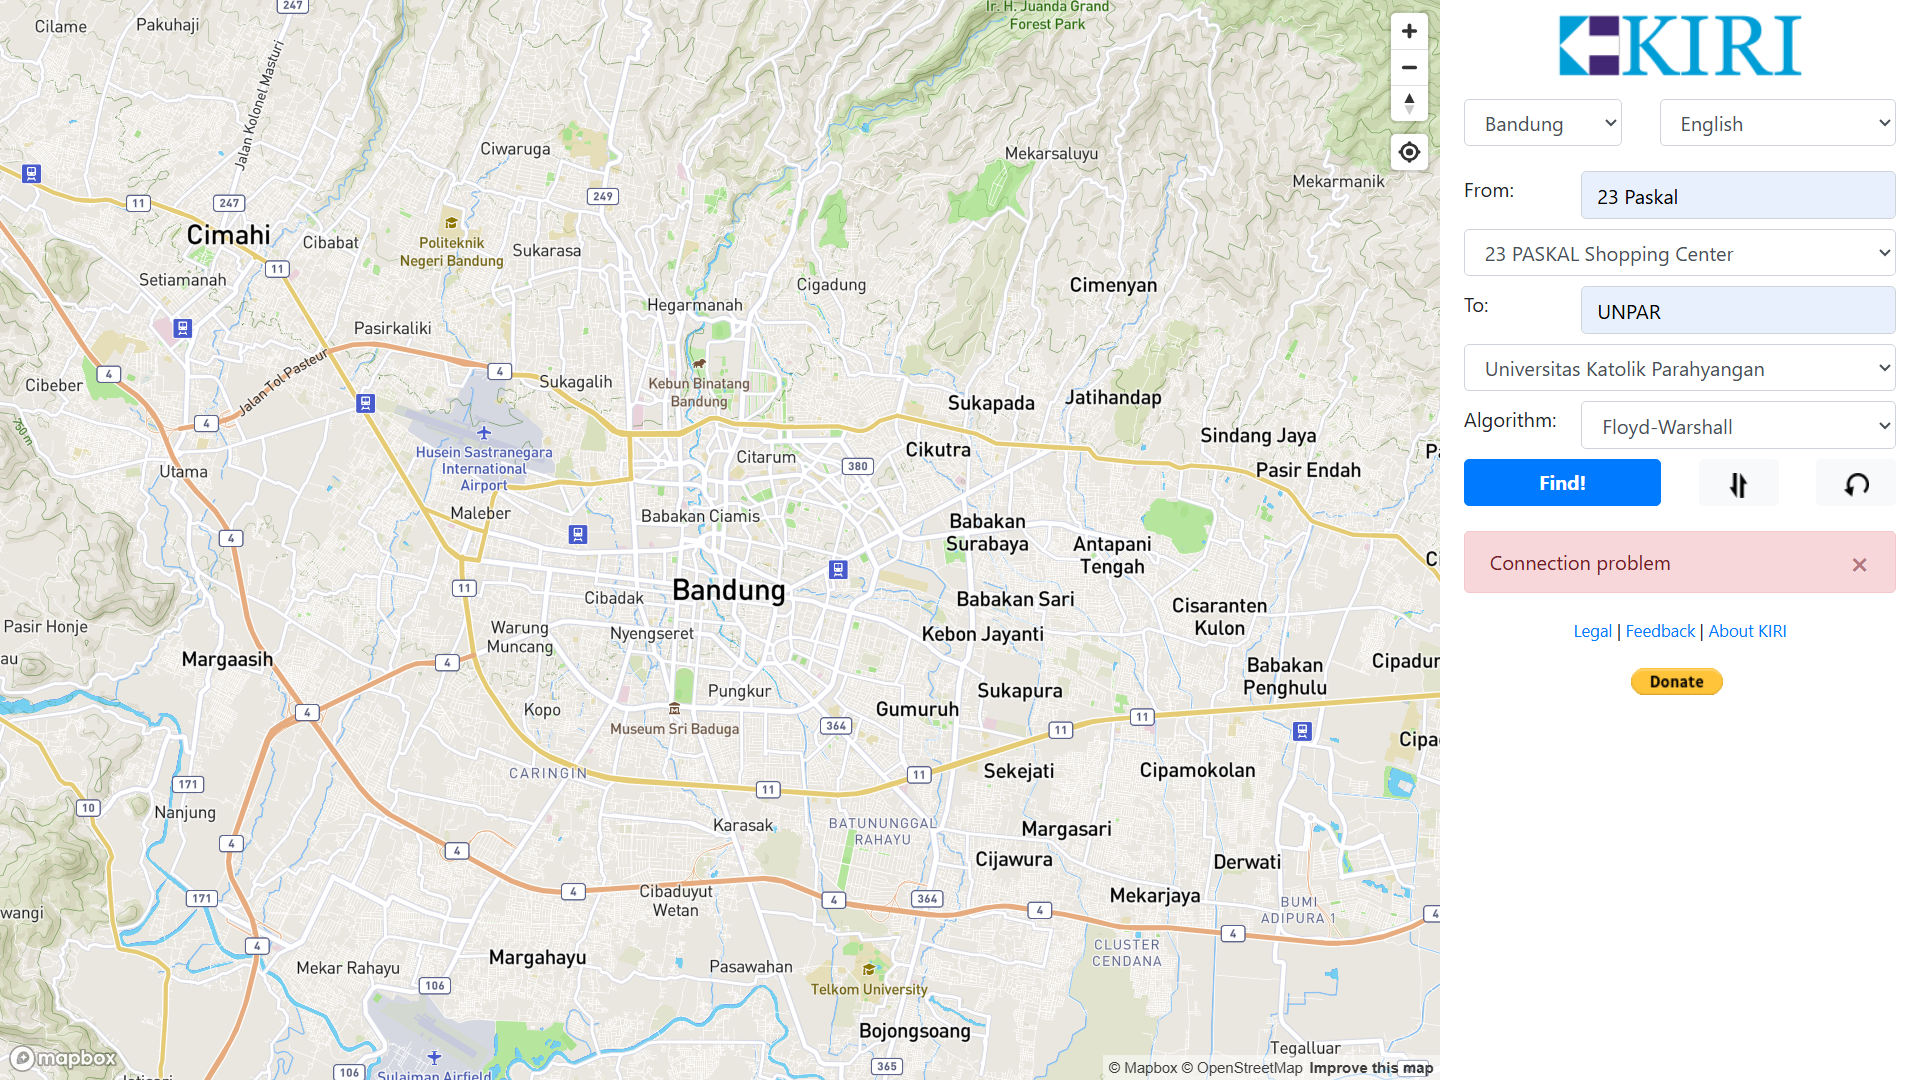
\includegraphics[width=1\textwidth]{error-1}
    \caption{Kondisi Saat Algoritma Floyd-Warshall Tidak Berhasil Dijalankan}
    \label{fig:error1}
\end{figure}

\begin{figure}[H]
    \centering
    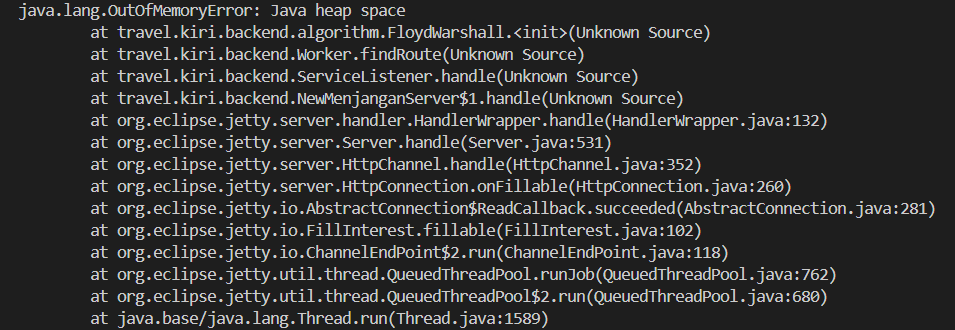
\includegraphics[width=1\textwidth]{error-2}
    \caption{Error Yang Menyebabkan Algoritma Floyd-Warshall Tidak Berhasil Dijalankan}
    \label{fig:error2}
\end{figure}

\noindent
Setelah dilakukan beberapa pengujian, jumlah data "tracks" yang dapat digunakan adalah lima record saja. Karena ketika jumlah data lebih dari lima record, pencarian jalur terpendek menggunakan algoritma Floyd-Warshall tidak berhasil dilakukan (lihat Gambar \ref{fig:error1}) yang disebabkan program mencoba menggunakan lebih banyak memori dari yang tersedia di heap \textit{Java Virtual Machine} (JVM) (lihat Gambar \ref{fig:error2}). Oleh karena itu, pada pengujian ini, jumlah data "tracks" yang akan digunakan adalah lima record, dengan data yang digunakan, yaitu Ciroyom - Antapani, Ciroyom - Ciburial, Ciumbuleuit - St. Hall (belok), Ciumbuleuit - St. Hall (lurus), dan Dago - Caringin.

\begin{comment}
\begin{table}[H]
\centering
\caption{Data Pengujian}
\label{tab:data}
{\large
\begin{tabular}{|l|l|}
\hline
\textbf{trackId}       & \textbf{trackName}             \\ \hline
ciroyomantapani & Ciroyom - Antapani \\ \hline
ciroyomciburial & Ciroyom - Ciburial \\ \hline
ciumbuleuitsthallbelok   & Ciumbuleuit - St. Hall (belok)     \\ \hline
ciumbuleuitsthalllurus        & Ciumbuleuit - St. Hall (lurus)             \\ \hline
dagocaringin        & Dago - Caringin             \\ \hline
\end{tabular}
}
\end{table}
\end{comment}

\subsubsection{Pengujian 1: Algoritma Dijkstra}
Hasil yang diharapkan dari pengujian menggunakan algoritma dijkstra ini adalah perangkat lunak KIRI dapat berjalan dengan tidak adanya error serta dapat ditemukannya jalur yang optimal. Pada pengujian ini menggunakan data sebagai berikut:
\begin{itemize}
    \item Titik awal: "23 Paskal"
    \item Titik akhir: "UNPAR"
    \item Algoritma: "Dijkstra"
\end{itemize}

\begin{figure}[H]
    \centering
    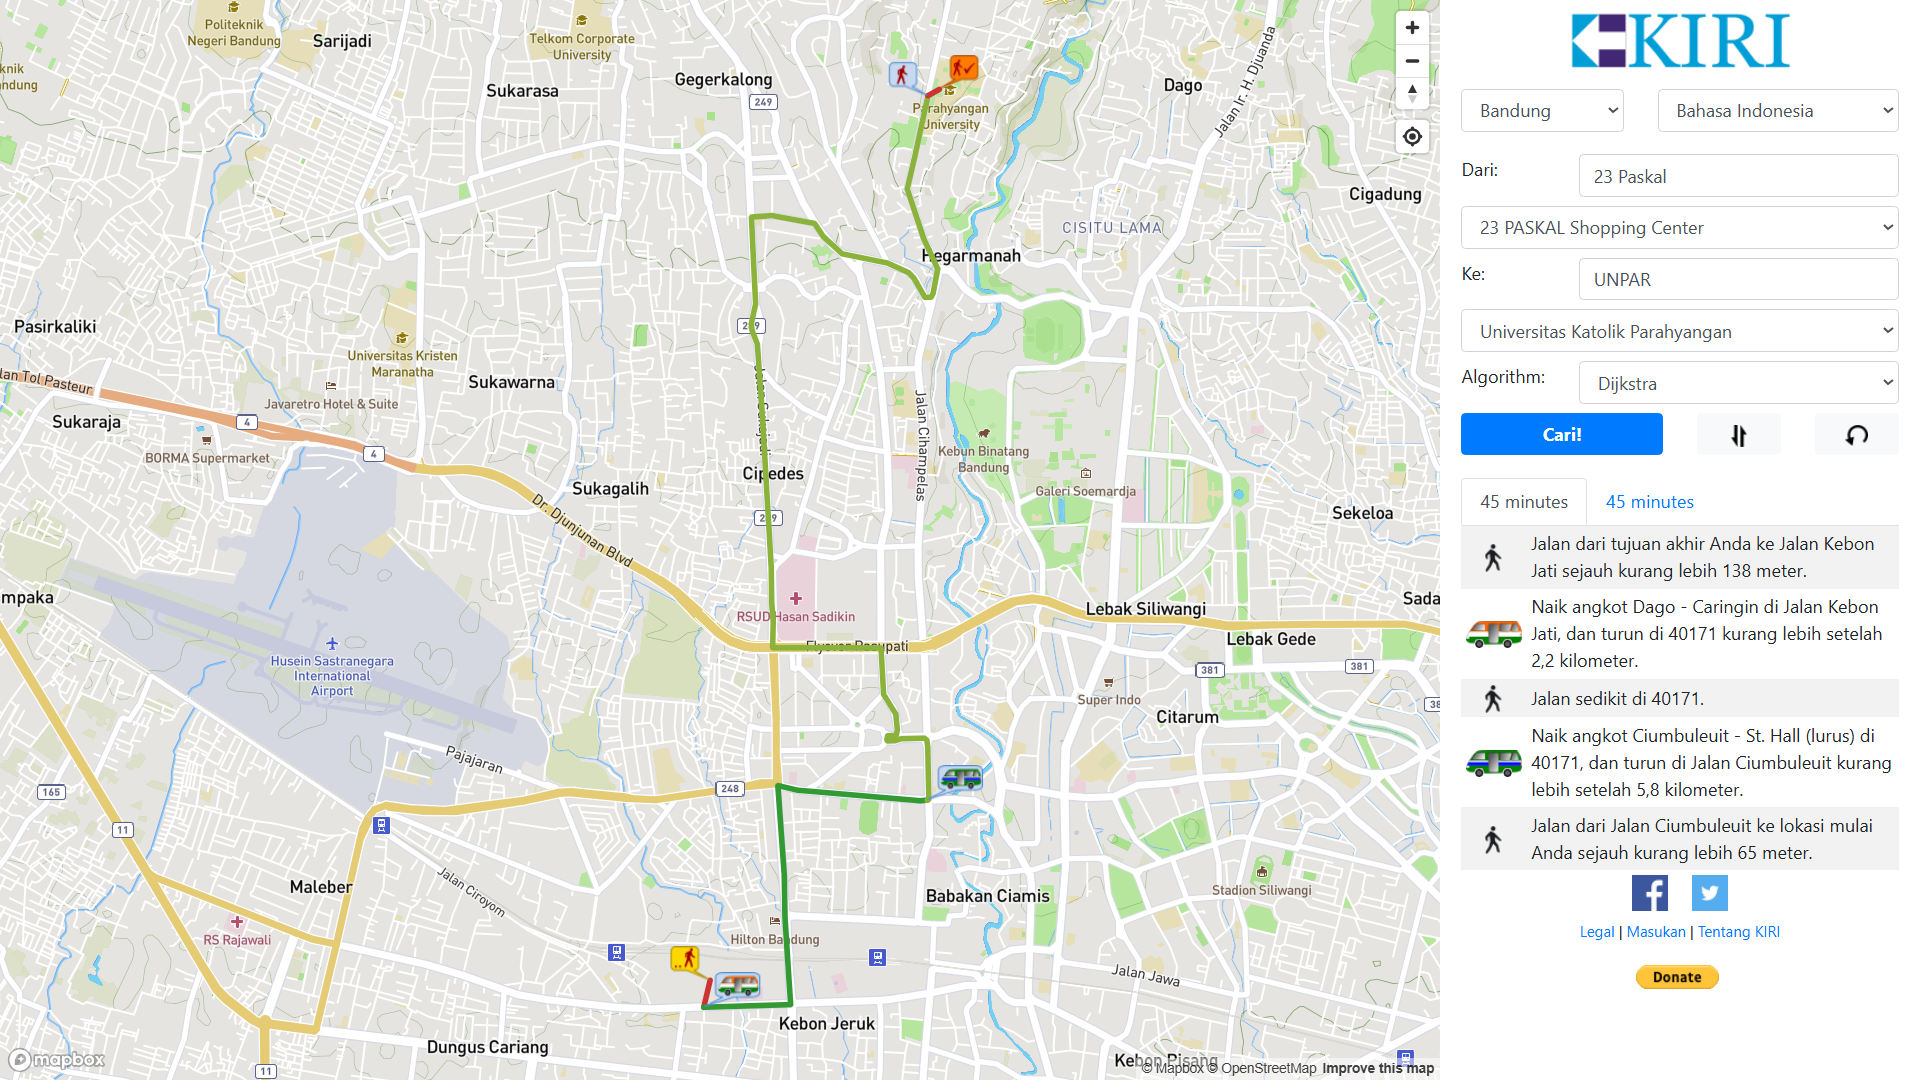
\includegraphics[width=0.8\textwidth]{hasil-dijkstra-1}
    \caption{Hasil Pengujian Algoritma Dijkstra Jalur 1}
    \label{fig:hasildijkstra-1}
\end{figure}

\begin{figure}[H]
    \centering
    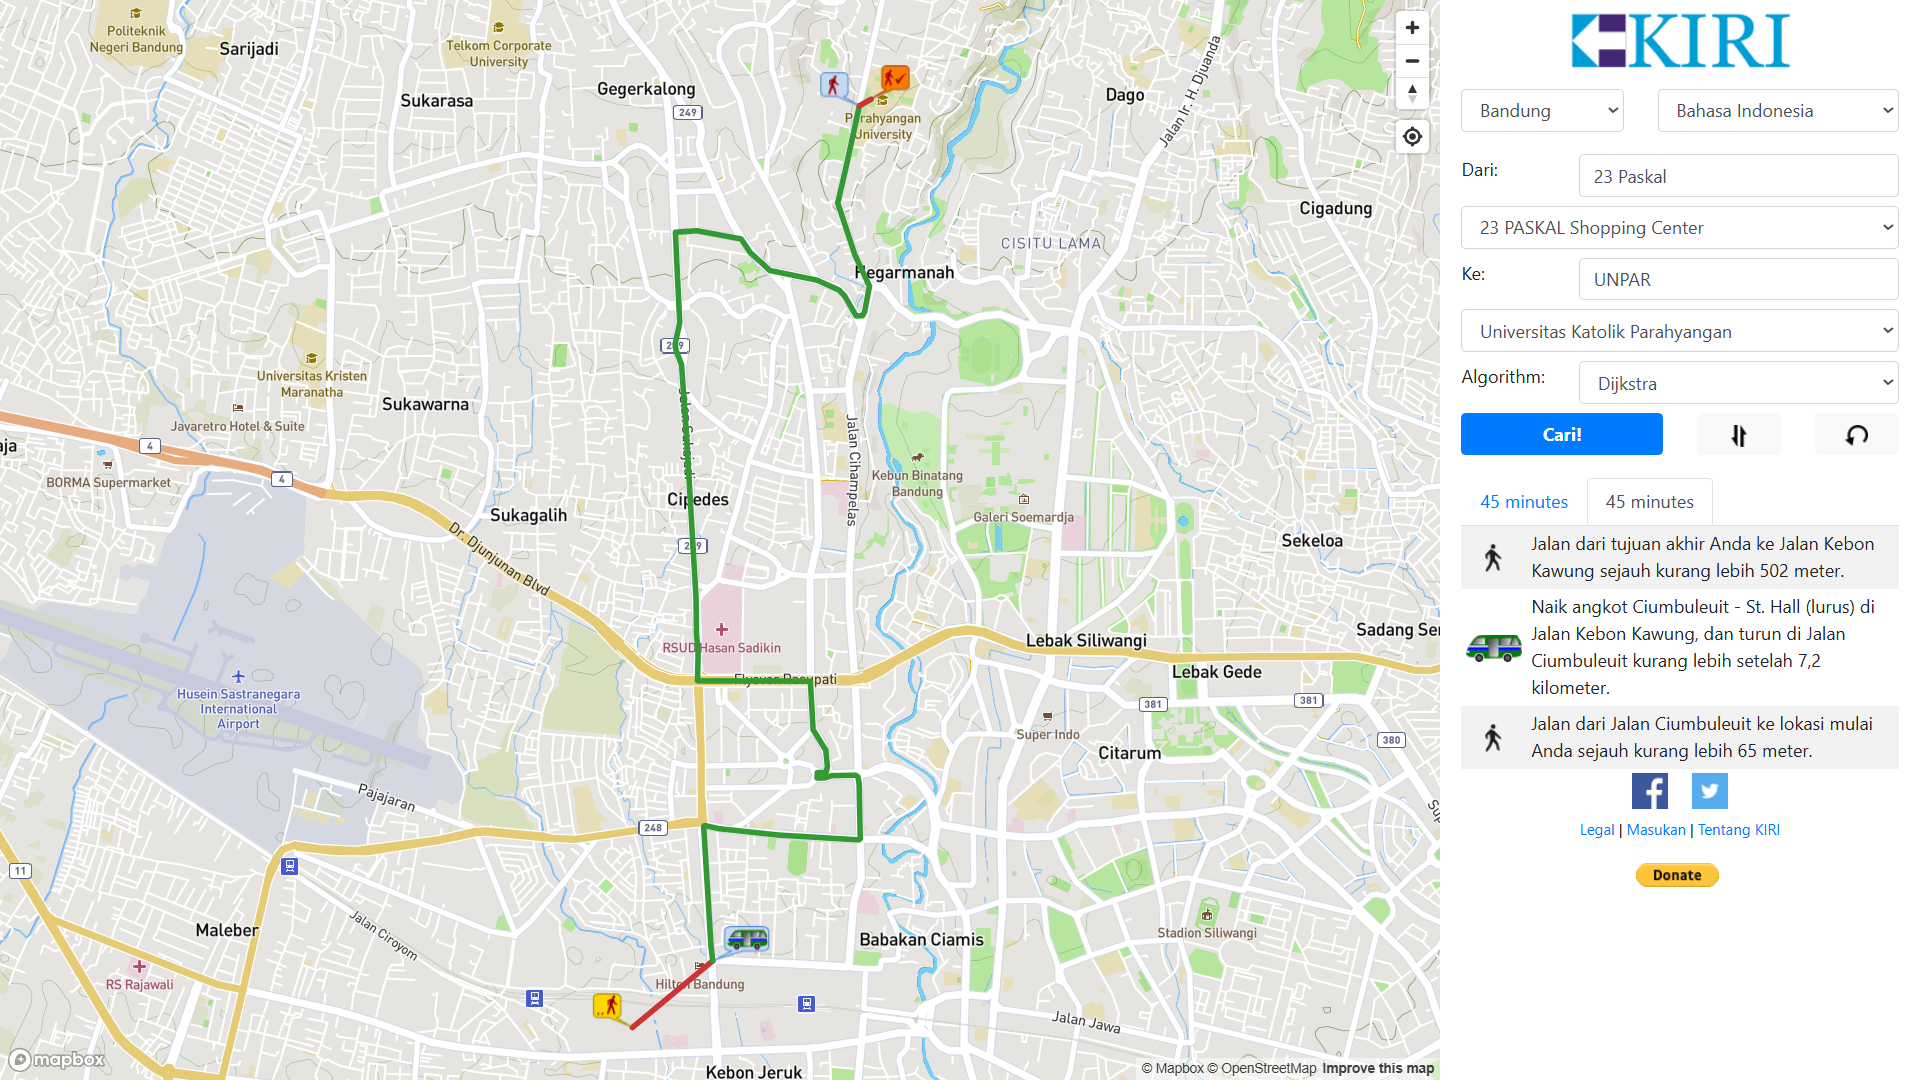
\includegraphics[width=0.8\textwidth]{hasil-dijkstra-2}
    \caption{Hasil Pengujian Algoritma Dijkstra Jalur 2}
    \label{fig:hasildijkstra-2}
\end{figure}
\noindent
Setelah semua data yang perlukan diisi dan dilakukan pencarian, perangkat lunak KIRI berjalan dengan baik ketika melakukan pencarian menggunakan algoritma Dijkstra, serta dapat menemukan dua jalur yang optimal dari Paskal 23 menuju UNPAR (lihat Gambar \ref{fig:hasildijkstra-1} dan \ref{fig:hasildijkstra-2}).

\subsubsection{Pengujian 2: Algoritma Floyd-Warshall}
Hasil yang diharapkan dari pengujian menggunakan algoritma Floyd-Warshall ini adalah perangkat lunak KIRI dapat berjalan dengan tidak adanya error serta dapat ditemukannya jalur yang optimal. Pada pengujian ini menggunakan data sebagai berikut:
\begin{itemize}
    \item Titik awal: "23 Paskal"
    \item Titik akhir: "UNPAR"
    \item Algoritma: "Floyd-Warshall"
\end{itemize}

\begin{figure}[H]
    \centering
    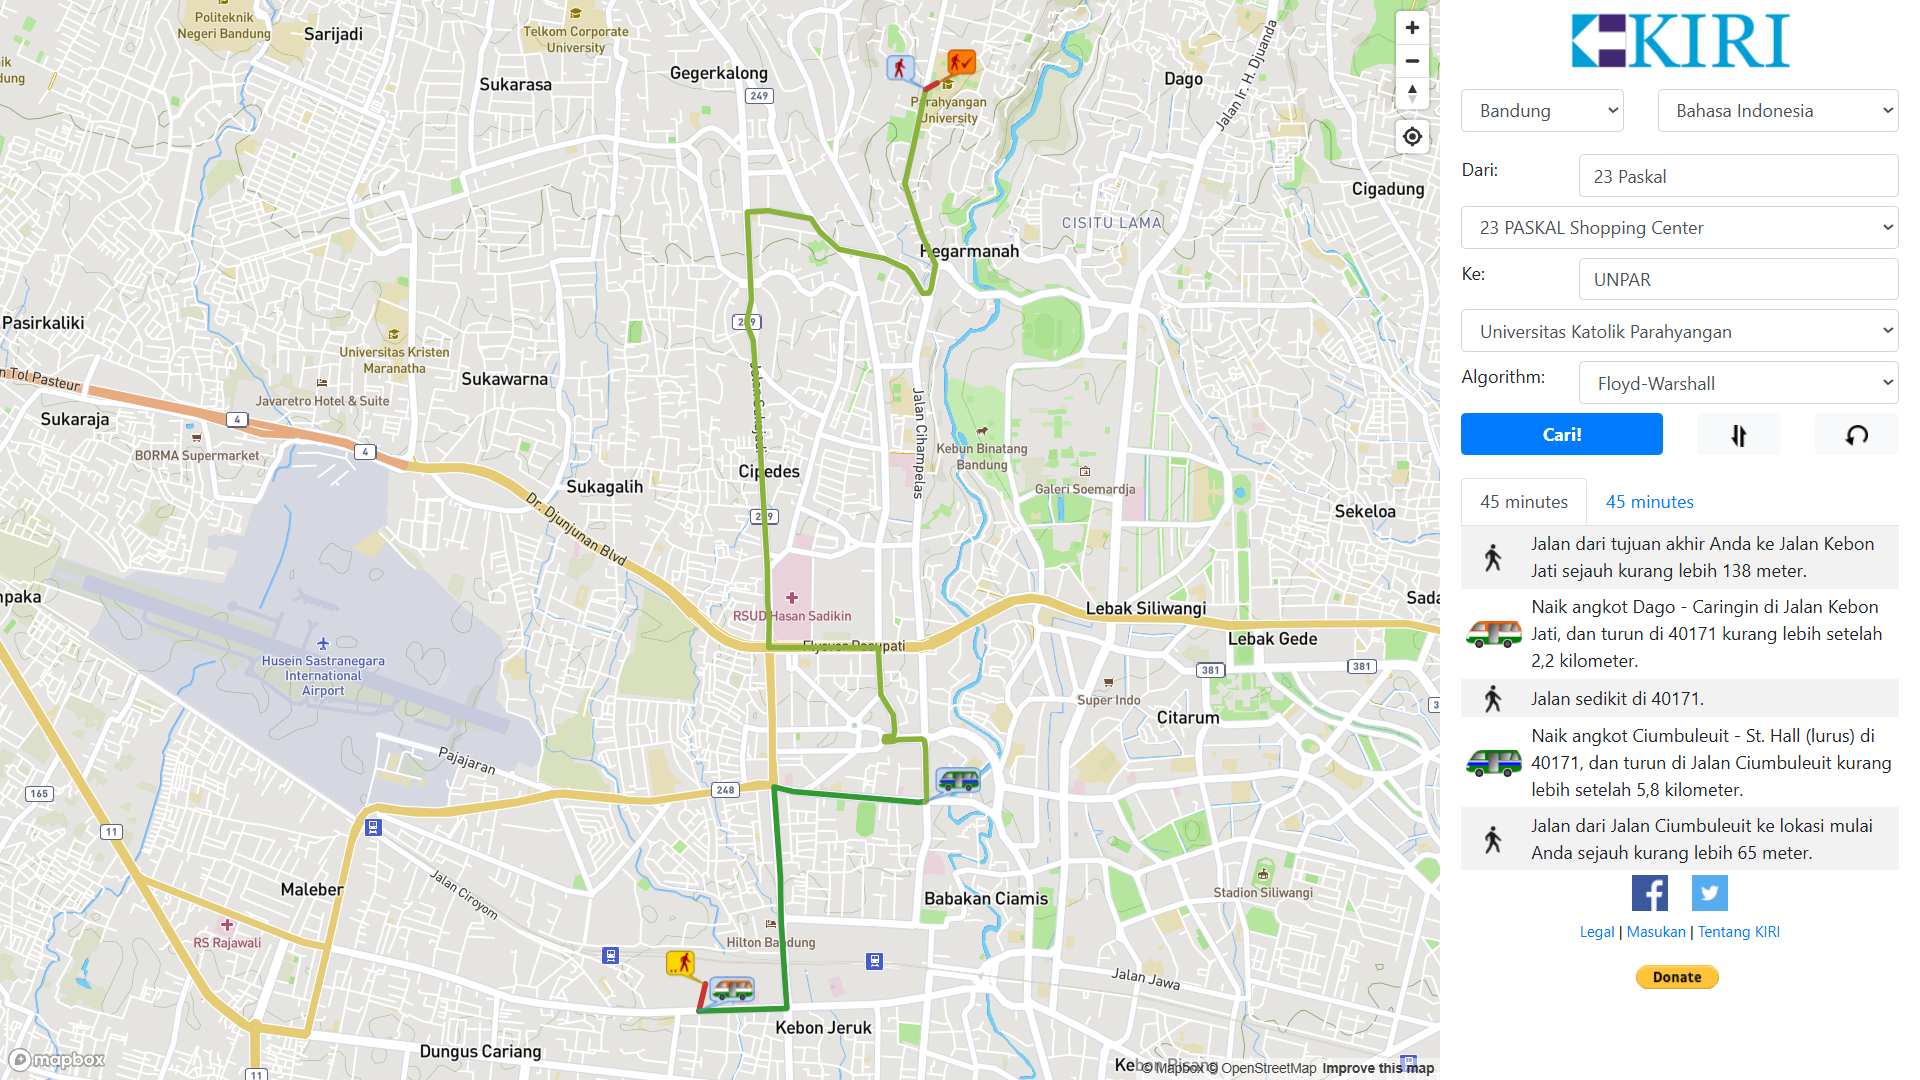
\includegraphics[width=0.8\textwidth]{hasil-floydwarshall-1}
    \caption{Hasil Pengujian Algoritma Floyd-Warshall Jalur 1}
    \label{fig:hasilfloydwarshall-1}
\end{figure}

\begin{figure}[H]
    \centering
    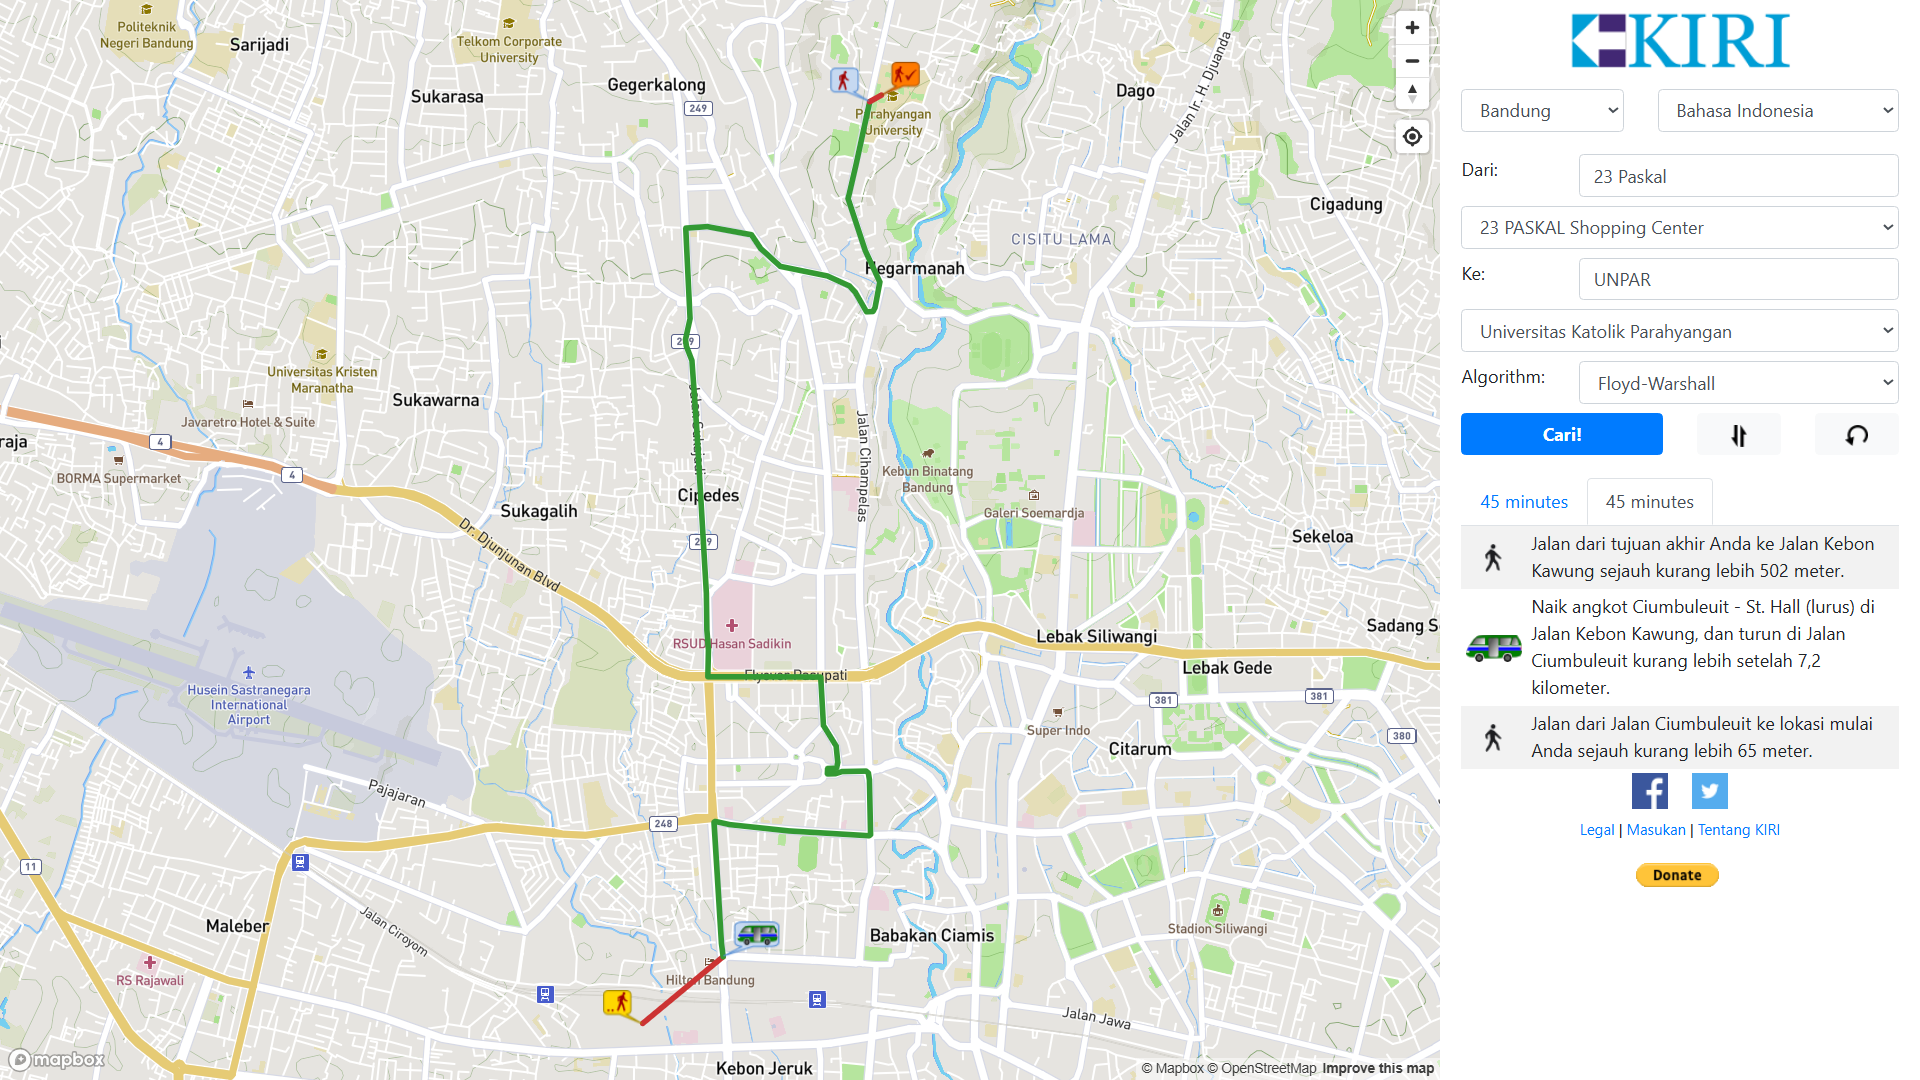
\includegraphics[width=0.8\textwidth]{hasil-floydwarshall-2}
    \caption{Hasil Pengujian Algoritma Floyd-Warshall Jalur 2}
    \label{fig:hasilfloydwarshall-2}
\end{figure}

\noindent
Setelah semua data yang perlukan diisi dan dilakukan pencarian, perangkat lunak KIRI berjalan dengan baik ketika melakukan pencarian menggunakan algoritma Floyd-Warshall tidak terjadi error atau gagal melakukan pencarian seperti pada gambar \ref{fig:error1} dan gambar \ref{fig:error2}, serta dapat menemukan dua jalur yang optimal dari Paskal 23 menuju UNPAR (lihat Gambar \ref{fig:hasilfloydwarshall-1} dan \ref{fig:hasilfloydwarshall-2}).

\subsubsection{Pengujian 3: Algoritma A-Star}
Hasil yang diharapkan dari pengujian menggunakan algoritma A-Star ini adalah perangkat lunak KIRI dapat berjalan dengan tidak adanya error serta dapat ditemukannya jalur yang optimal. Pada pengujian ini menggunakan data sebagai berikut:
\begin{itemize}
    \item Titik awal: "23 Paskal"
    \item Titik akhir: "UNPAR"
    \item Algoritma: "A-Star"
\end{itemize}

\begin{figure}[H]
    \centering
    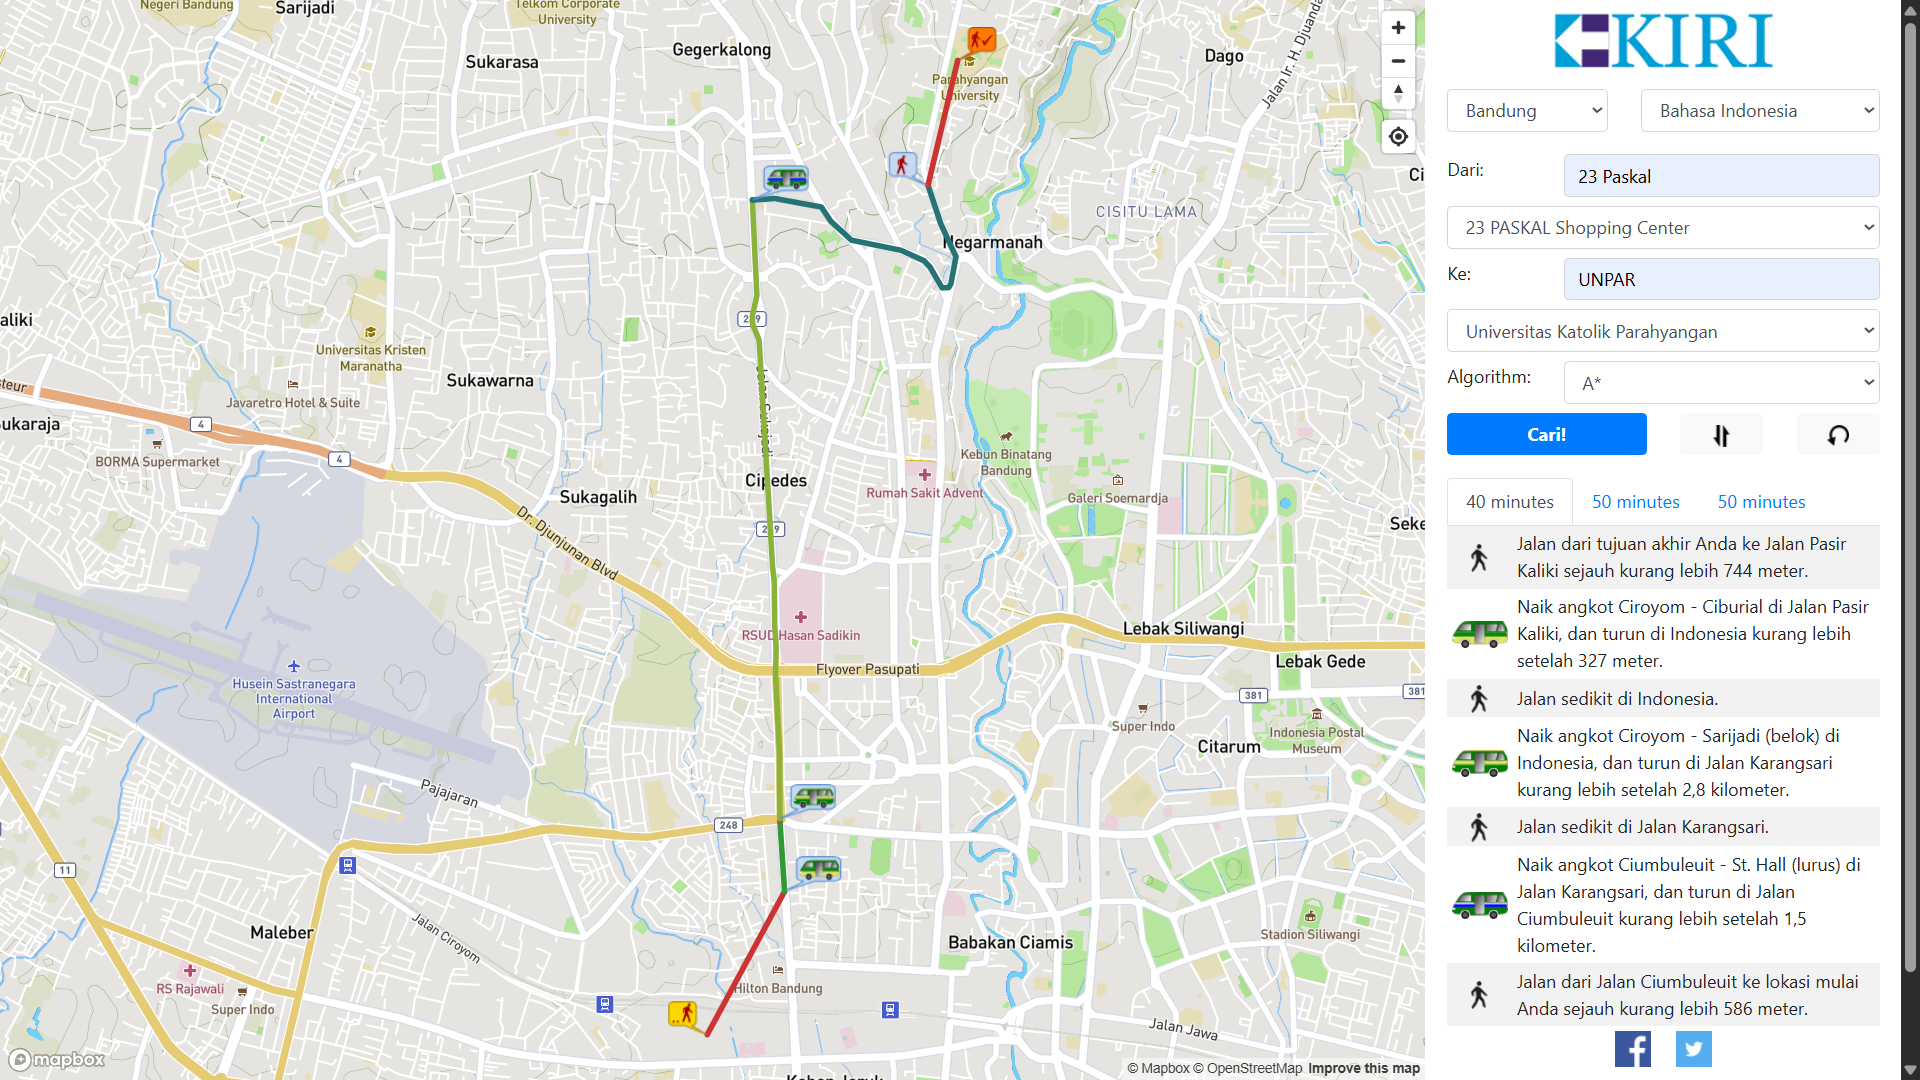
\includegraphics[width=0.8\textwidth]{hasil-astar-1}
    \caption{Hasil Pengujian Algoritma A-Star Jalur 1}
    \label{fig:hasilastar1}
\end{figure}

\begin{figure}[H]
    \centering
    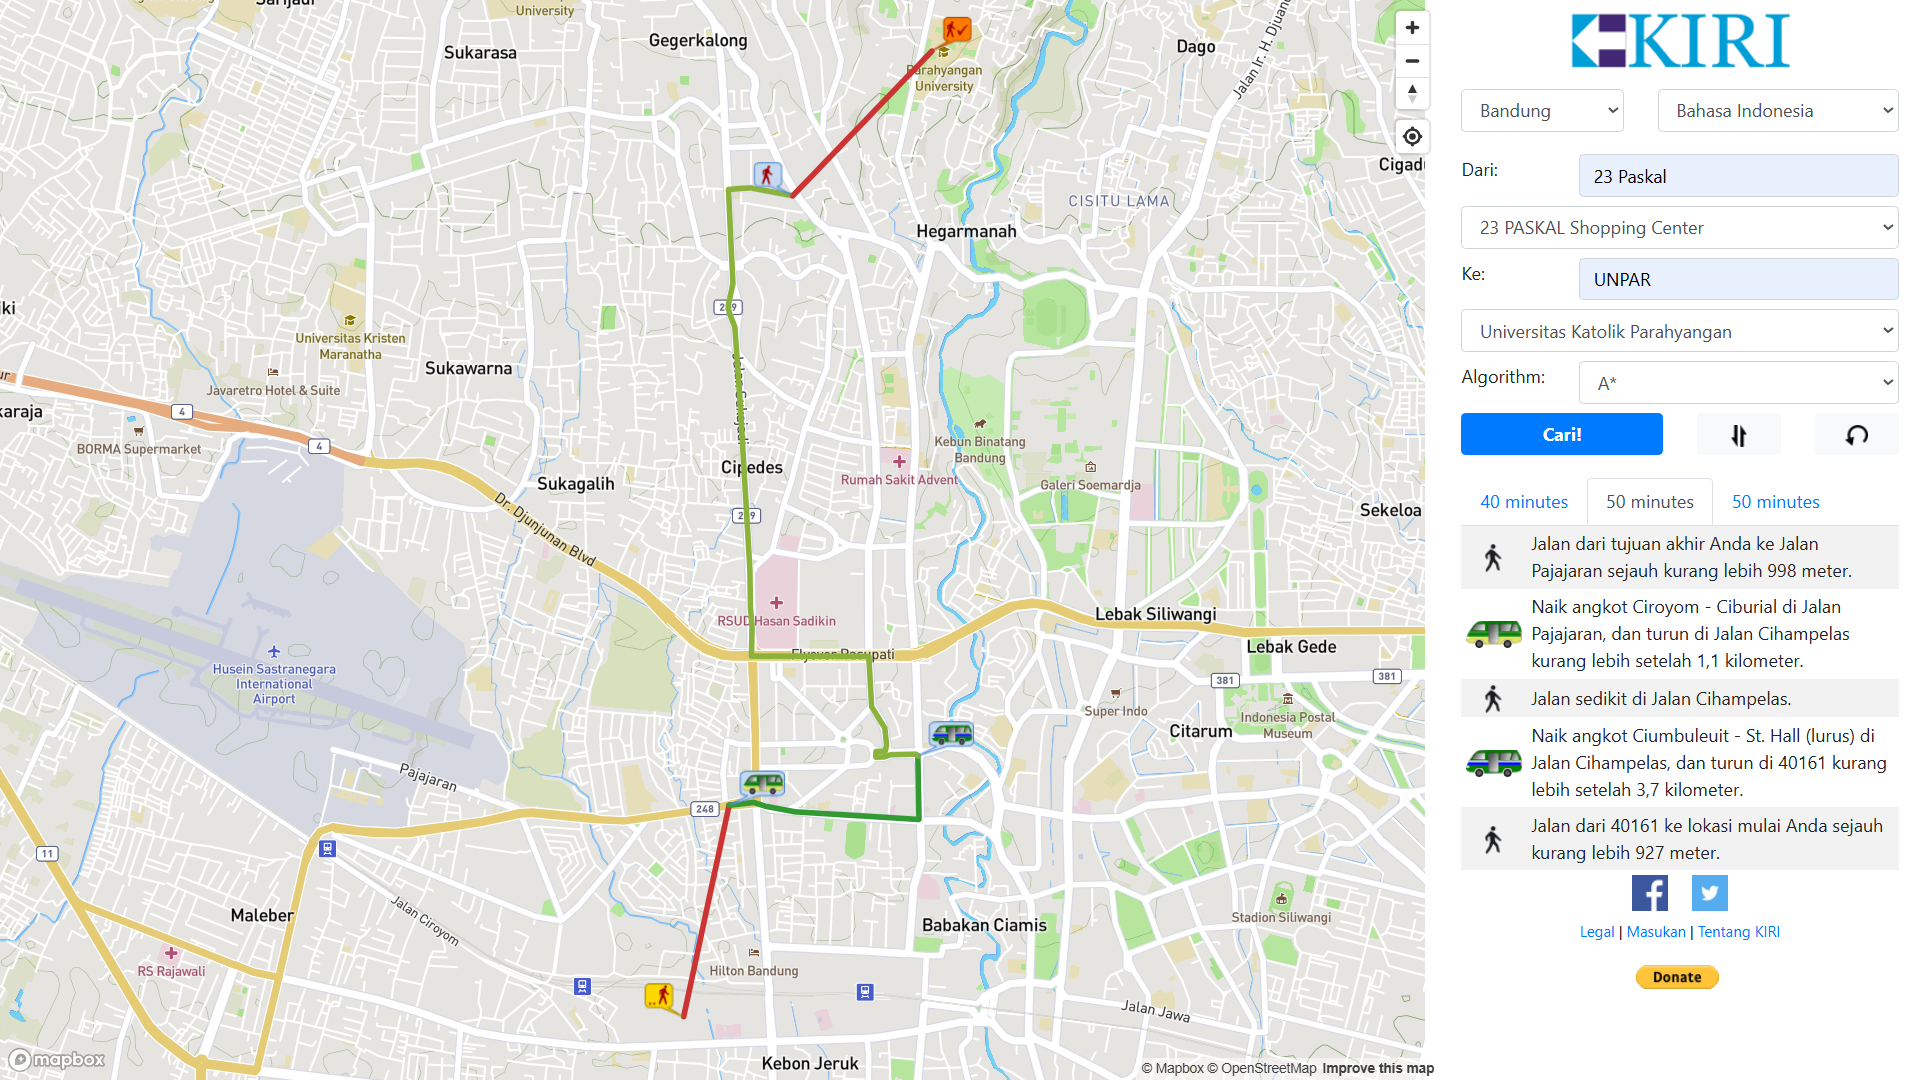
\includegraphics[width=0.8\textwidth]{hasil-astar-2}
    \caption{Hasil Pengujian Algoritma A-Star Jalur 2}
    \label{fig:hasilastar2}
\end{figure}

\noindent
Setelah semua data yang perlukan diisi dan dilakukan pencarian, perangkat lunak KIRI berjalan dengan baik ketika melakukan pencarian menggunakan algoritma A-Star, serta dapat menemukan dua jalur yang optimal dari Paskal 23 menuju UNPAR(lihat Gambar \ref{fig:hasilastar1} dan \ref{fig:hasilastar2}).

\subsection{Pengujian Eksperimental}
\label{subsec:pengujianeksperimental}
Pengujian akan dilakukan untuk mengukur waktu eksekusi untuk setiap algoritma yang sudah diimplementasikan dalam melakukan pencarian atau perhitungan jalur terpendek dari titik awal hingga titik tujuan. Sebelum dilakukan pengujian, berikut disajikan kompleksitas waktu dari masing-masing algoritma untuk dijadikan sebagai acuan.
\begin{itemize}
    \item Algoritma Dijkstra: $O((V+E)$ $log$ $V)$.
    \item Algoritma A-Star: $O((V+E)$ $log$ $V)$.
    \item Algoritma Floyd-Warshall: $O(V^3)$.
\end{itemize}
\noindent
Pengujian ini akan dibagi menjadi dua bagian, bagian pertama hanya akan menggunakan lima record dari data "tracks" saja dan seluruh algoritma akan diuji, sedangkan pada bagian kedua akan digunakan seluruh record pada data "tracks" dan hanya algoritma Dijkstra dan A-Star saja yang akan diuji. Selain itu, untuk setiap algoritmanya akan diuji sebanyak tiga kali dan juga untuk setiap bagiannya akan terdapat tiga kasus yang berbeda. Rangkuman kasus-kasus dari pengujian yang akan dilakukan dapat dilihat pada tabel \ref{tab:rangkumankasus}.
\\
Pada pengujian ini, pengukuran waktu menggunakan \texttt{System.nanoTime()} sebelum proses pencarian jalur dimulai dan diakhiri dengan mencatat waktu akhir setelah seluruh proses pencarian dan pembentukan hasil selesai. Selisih antara waktu akhir dan waktu awal dihitung dan dikonversi dari nanodetik ke milidetik dengan membaginya sebesar 1.000.000. Pengukuran ini dilakukan pada kelas \texttt{Worker.java} yang kodenya bisa dilihat pada \ref{code:worker}.

\renewcommand{\arraystretch}{1.5}
\begin{table}[H]
\caption{Rangkuman Kasus Pengujian}
{\large
\label{tab:rangkumankasus}
\begin{tabular}{|l|l|l|l|}
\hline
{\textbf{Pengujian}} & {\textbf{Titik Awal}} & {\textbf{Titik Akhir}} & {\textbf{Tracks}}                                                                                                                                     \\ \hline
1.1                                      & 23 Paskal                                & UNPAR                                     & \begin{tabular}[c]{@{}l@{}}Ciroyom - Antapani\\ Ciroyom - Ciburial\\ Ciumbuleuit - St. Hall (belok)\\ Ciumbuleuit - St. Hall (lurus)\\ Dago - Caringin\end{tabular}      \\ \hline
1.2                                      & Gedung Sate                              & Trans Studio Bandung                      & \begin{tabular}[c]{@{}l@{}}Cicadas - Elang (Kalapa - Cicadas)\\ Cicadas - Elang (Kalapa - Elang)\\ Dago - Caringin\\ Dago - Riung Bandung\\ Kalapa - Ledeng\end{tabular} \\ \hline
1.3                                      & Alun-Alun Bandung                        & Festival Citylink                         & \begin{tabular}[c]{@{}l@{}}Cijerah - Ciwastra\\ Kalapa - Buah Batu\\ Kalapa - Cibaduyut\\ Kalapa - Karang Setra\\ Kalapa - Ledeng\end{tabular}                           \\ \hline
2.1                                      & 23 Paskal                                & UNPAR                                     & Seluruh tracks digunakan                                                                                                                                                 \\ \hline
2.2                                      & Gedung Sate                              & Trans Studio Bandung                      & Seluruh tracks digunakan                                                                                                                                                 \\ \hline
2.3                                      & Alun-Alun Bandung                        & Festival Citylink                         & Seluruh tracks digunakan                                                                                                                                                 \\ \hline
\end{tabular}
}
\end{table}

\subsubsection{Pengujian 1.1}
Pada pengujian ini titik awal yang digunakan, yaitu "23 Paskal" dan titik akhir, yaitu "UNPAR". Selain itu, pada pengujian ini data "tracks" yang digunakan, yaitu Ciroyom - Antapani, Ciroyom - Ciburial, Ciumbuleuit - St. Hall (belok), Ciumbuleuit - St. Hall (lurus), dan Dago - Caringin.

\begin{comment}
\begin{table}[H]
\centering
\caption{Data Pengujian 1.1}
\label{tab:data1.1}
{\large
\begin{tabular}{|l|l|}
\hline
\textbf{trackId}       & \textbf{trackName}             \\ \hline
ciroyomantapani & Ciroyom - Antapani \\ \hline
ciroyomciburial & Ciroyom - Ciburial \\ \hline
ciumbuleuitsthallbelok   & Ciumbuleuit - St. Hall (belok)     \\ \hline
ciumbuleuitsthalllurus        & Ciumbuleuit - St. Hall (lurus)             \\ \hline
dagocaringin        & Dago - Caringin             \\ \hline
\end{tabular}
}
\end{table}
\end{comment}

\renewcommand{\arraystretch}{1.8}
\begin{table}[H]
\centering
\caption{Hasil Pengujian 1.1}
\label{tab:hasiluji1.1}
{\large
\begin{tabular}{|l|r|r|r|r|} 
\hline
{\textbf{Algoritma}} & {\textbf{Pengujian 1}} & {\textbf{Pengujian 2}} & {\textbf{Pengujian 3}} & \multicolumn{1}{l|}{\textbf{Average}} \\ 
\hline
Dijkstra       & 3.43 ms              & 4.29 ms              & 4.23 ms              & 3.98 ms          \\
\hline
A-Star         & 4.09 ms              & 3.96 ms              & 4.37 ms              & 4.14 ms          \\
\hline
Floyd-Warshall & 26469.95 ms          & 25765.38 ms          & 27804.94 ms          & 26680.09 ms \\
\hline
\end{tabular}
}
\end{table}

\subsubsection{Pengujian 1.2}
Pada pengujian ini titik awal yang digunakan, yaitu "Gedung Sate" dan titik akhir, yaitu "Trans Studio Bandung". Selain itu, pada pengujian ini data "tracks" yang digunakan, yaitu Cicadas - Elang (Kalapa - Cicadas), Cicadas - Elang (Kalapa - Elang), Dago - Caringin, Dago - Riung Bandung, dan Kalapa - Ledeng.

\begin{comment}
\begin{table}[H]
\centering
\caption{Data Pengujian 1.2}
\label{tab:data1.2}
{\large
\begin{tabular}{|l|l|}
\hline
\textbf{trackId}       & \textbf{trackName}             \\ \hline
cicadaselangkalapacicadas & Cicadas - Elang (Kalapa - Cicadas) \\ \hline
cicadaselangkalapaelang & Cicadas - Elang (Kalapa - Elang) \\ \hline
dagocaringin   & Dago - Caringin     \\ \hline
dagoriungbandung        & Dago - Riung Bandung             \\ \hline
kalapaledeng        & Kalapa - Ledeng             \\ \hline
\end{tabular}
}
\end{table}
\end{comment}

\begin{table}[H]
\centering
\caption{Hasil Pengujian 1.2}
\label{tab:hasiluji1.2}
{\large
\begin{tabular}{|l|r|r|r|r|}
\hline
\textbf{Algoritma} & \textbf{Pengujian 1} & \textbf{Pengujian 2} & \textbf{Pengujian 3} & \multicolumn{1}{l|}{\textbf{Average}}\\ \hline
Dijkstra           & 3.17 ms              & 3.66 ms             & 3.22 ms       &       3.35 ms             \\ \hline
A-Star            & 3.30 ms              & 3.19 ms              & 3.49 ms       &       3.32 ms             \\ \hline
Floyd-Warshall     & 31212.38 ms              & 30494.62 ms               & 30710.07 ms     &   30804.69 ms            \\ \hline
\end{tabular}
}
\end{table}

\subsubsection{Pengujian 1.3}
Pada pengujian ini titik awal yang digunakan, yaitu "Alun-Alun Bandung" dan titik akhir, yaitu "Festival Citylink". Selain itu, pada pengujian ini data "tracks" yang digunakan, yaitu Cijerah - Ciwastra, Kalapa - Buah Batu, Kalapa - Cibaduyut, Kalapa - Karang Setra, dan Kalapa - Ledeng.

\begin{comment}
\begin{table}[H]
\centering
\caption{Data Pengujian 1.3}
\label{tab:data1.3}
{\large
\begin{tabular}{|l|l|}
\hline
\textbf{trackId}       & \textbf{trackName}             \\ \hline
cijerahciwastra & Cijerah - Ciwastra \\ \hline
kalapabuahbatu & Kalapa - Buah Batu \\ \hline
kalapacibaduyut   & Kalapa - Cibaduyut     \\ \hline
kalapakarangsetra        & Kalapa - Karang Setra             \\ \hline
kalapaledeng        & Kalapa - Ledeng             \\ \hline
\end{tabular}
}
\end{table}
\end{comment}

\begin{table}[H]
\centering
\caption{Hasil Pengujian 1.3}
\label{tab:hasiluji1.3}
{\large
\begin{tabular}{|l|r|r|r|r|}
\hline
\textbf{Algoritma} & \textbf{Pengujian 1} & \textbf{Pengujian 2} & \textbf{Pengujian 3} & \multicolumn{1}{l|}{\textbf{Average}}\\ \hline
Dijkstra           & 2.31 ms              & 2.18 ms             & 1.96 ms      &    2.15 ms           \\ \hline
A-Star            & 2.42 ms              & 2.29 ms              & 2.26 ms      &    2.32 ms        \\ \hline
Floyd-Warshall     & 8799.05 ms              & 6577.51 ms               & 8568.48 ms      &     7981.68 ms        \\ \hline
\end{tabular}
}
\end{table}

\subsubsection{Pengujian 2.1}
Pada pengujian ini titik awal yang digunakan, yaitu "23 Paskal" dan titik akhir, yaitu "UNPAR". Selain itu, pada pengujian ini seluruh data "tracks" digunakan.

\begin{table}[H]
\centering
\caption{Hasil Pengujian 2.1}
\label{tab:hasiluji2.1}
{\large
\begin{tabular}{|l|r|r|r|r|}
\hline
\textbf{Algoritma} & \textbf{Pengujian 1} & \textbf{Pengujian 2} & \textbf{Pengujian 3} & {\textbf{Average}}\\ \hline
Dijkstra           & 44.45 ms              & 46.98 ms             & 46.22 ms     &      45.88 ms         \\ \hline
A-Star            & 26.65 ms              & 30.02 ms              & 27.30 ms      &      27.99 ms        \\ \hline
\end{tabular}
}
\end{table}

\subsubsection{Pengujian 2.2}
Pada pengujian ini titik awal yang digunakan, yaitu "Gedung Sate" dan titik akhir, yaitu "Trans Studio Bandung". Selain itu, pada pengujian ini seluruh data "tracks" digunakan.

\begin{table}[H]
\centering
\caption{Hasil Pengujian 2.2}
\label{tab:hasiluji2.2}
{\large
\begin{tabular}{|l|r|r|r|r|}
\hline
\textbf{Algoritma} & \textbf{Pengujian 1} & \textbf{Pengujian 2} & \textbf{Pengujian 3} & {\textbf{Average}}\\ \hline
Dijkstra           & 83.23 ms              & 75.47 ms             & 80.42 ms       &       79.70 ms       \\ \hline
A-Star            & 28.45 ms              & 26.56 ms              & 27.61 ms      &      27.54 ms       \\ \hline
\end{tabular}
}
\end{table}

\subsubsection{Pengujian 2.3}
Pada pengujian ini titik awal yang digunakan, yaitu "Alun-Alun Bandung" dan titik akhir, yaitu "Festival Citylink". Selain itu, pada pengujian ini seluruh data "tracks" digunakan.

\begin{table}[H]
\centering
\caption{Hasil Pengujian 2.3}
\label{tab:hasiluji2.3}
{\large
\begin{tabular}{|l|r|r|r|r|}
\hline
\textbf{Algoritma} & \textbf{Pengujian 1} & \textbf{Pengujian 2} & \textbf{Pengujian 3} & \multicolumn{1}{l|}{\textbf{Average}}\\ \hline
Dijkstra           & 52.30 ms              & 51.21 ms             & 49.21 ms      &     50.90 ms        \\ \hline
A-Star            & 34.76 ms              & 31.64 ms              & 33.47 ms      &     33.29 ms        \\ \hline
\end{tabular}
}
\end{table}

\subsubsection{Kesimpulan Pengujian}
\noindent
Berdasarkan hasil pengujian 1 yang bisa dilihat pada tabel \ref{tab:hasiluji1.1}, \ref{tab:hasiluji1.2}, dan \ref{tab:hasiluji1.3}, algoritma Dijkstra dan A-Star memiliki waktu eksekusi yang relatif sama. Akan tetapi, algoritma Floyd-Warshall memiliki waktu eksekusi yang cukup besar dibanding kedua algoritma lainnya, hal tersebut disebabkan karena algoritma Floyd-Warshall memiliki kompleksitas waktu yang sangat besar dan jauh lebih besar dari pada dua algoritma lainnya, serta Floyd-Warshall juga memanfaatkan matriks sehingga simpul yang diproses pun menjadi lebih banyak. Sedangkan, pada pengujian 2 algoritma A-Star memiliki waktu eksekusi yang lebih cepat dari algoritma Dijkstra berdasarkan seluruh pengujian dilakukan yang hasilnya bisa dilihat pada tabel \ref{tab:hasiluji2.1}, \ref{tab:hasiluji2.2}, dan \ref{tab:hasiluji2.3}. Meskipun kompleksitas waktu algoritma A-Star dan Dijkstra sama, tetapi algoritma A-Star bisa lebih cepat dibanding algoritma Dijkstra karena algoritma A-Star menggunakan fungsi heuristik. Dengan adanya heuristik ini, algoritma A-Star tidak perlu memproses semua simpul, melainkan hanya simpul-simpul yang dianggap lebih potensial berdasarkan nilai heuristicnya. Hal ini membuat jumlah simpul yang diproses menjadi lebih sedikit, sehingga berdampak pada waktu eksekusi yang lebih cepat.